\chapter{Results}
\label{chap:results}

As described in Section~\ref{sec:methodology}, a set of experiments was performed on the Kubernetes environment with a variety of pre-planted security misconfigurations. Since Kubernetes API Server Vulnerabilities from the Tab~\ref{tab:kubernetes-security-threat-classification} cannot be implemented in the local Rancher Desktop instance due to the Rancher Desktop's limited cluster configuration options, Tab~\ref{tab:kubernetes-security-threat-results} provides only data declared by the scanner documentation in this row.

If we look at the Trivy column, we can see that Trivy does not check for missing Pod Security Admission labels on the namespaces, which can be configured to reject pods with policy violations. Then, Trivy does not check for the missing Network Policies. According to the Aqua Vulnerability database \cite{aqua-vulnerability-database}, such check exists, but only for clusters deployed using Microsoft Azure services. Furthermore, Trivy does not check for missing of misconfigured Pod Preemption Policies, which bear a risk, according to the Kuberntes documentation \cite{pod-security-preemption}: ``a malicious user could create Pods at the highest possible priorities, causing other Pods to be evicted/not get scheduled.'' Trivy shows good performance in search for container vulnerabilities. It has detected the use of \textbf{latest} tag and found over a thousand package vulnerabilities inside the containers. However, it did not detect an exposed secret inside the container when executed in cluster scan mode. A separate execution specifically against the image registry has detected the secret. Trivy does not perform any networking checks, unnecessarily exposed services via LoadBalancer did not produce any warnings or failures, but binding of the container port to the host port on the Kubernetes Load Balancer workload has been detected. When it comes to the elevated pod privileges, Trivy was able to detect containers running as root and pods with added capabilties.

Kube-bench performs a pure CIS Kubernetes Benchmark scanning and, thus, does not include any additional checks for missing policies or resource limits. It is not able to perform container image scanning and, therefore, lacks any vulnerability output. Most of the scan results also require manual confirmation. That is, of 59 performed checks only 18 were automated. Moreover, Kube-bench was not able to perform any Control Plane or etcd benchmarks. It has recognized the only Rancher Desktop node as a Woker Node, thus, only executing Worker Node and Policies benchmarks.

Kubescape has yielded the best results overall. It is the only scanner from the selection that has checks for missing Pod Security Admission and Network policies. It is also the only scanner able to detect misconfigured ingress and egress controls. However, user has to explicitly include those into scanning process as these checks are not performed by the default scan.

Prowler does a great job in looking for misconfigured RBAC, there are 338 checks that detect vulnerabilities in RBAC resources. However, Prowler has no checks for resource limits or any securirity policies. It also cannot scan for any container vulnerabilities or misconfigured network policies. Prowler has a check for secrets as environment variables, but it did not recognize our pre-planted exposed secret as a misconfiguration. There are 9 manual checks for critical file ownership and auditing of the cluster roles.

Table~\ref{tab:kubernetes-security-threat-results} shows that all selected tools lack security coverage in some areas. None of the selected tools are able to detect missing or misconfigured Pod Preemption policies or detect exposed secrets in container images from a cluster scan. The former allows Kubernetes to schedule privileged pods and is of minor importance as scheduled privileged pods are still detected by the scanners. The latter, however, bears a major risk of becoming a critical vulnerability opening up the infrastructure for a potential attack. On the other hand, most of the modern container regisrties include a vulnerability scanner, which should be able to detect such threats.

Kubescape detects most of the security threats in different categories. Unfortunately, Kubescape does not yet support control extension with custom frameworks. There is some degree of customization as the user can extend the existing frameworks with custom checks, which he ``builds'' from the limited amount of predefined configuration parameters. That is, it is currently not possible to extend Kubescape's capabilities to make it scan for missing pod preemption policies or exposed secrets.

\begin{table}[H]
    \begin{center}
        \begin{tabular}{ | p{.25\textwidth} | p{.25\textwidth} | p{.10\textwidth} | p{.10\textwidth} | p{.10\textwidth} | p{.10\textwidth} | } 
        \hline
        Category & Subcategory & Trivy & Kube-bench & Kube-scape & Prowler \\ [0.5ex] 
        \hline\hline
        \multirow{5}{*}{} 1. Configuration Vulnerabilities & 1.1 Misconfigured RBAC & yes & yes & yes & yes \\ \cline{2-6} 
                & 1.2 Pod Security Admission & no & no & yes & no \\ \cline{2-6} 
                & 1.3 Network Policies & no & no & yes & no \\ \cline{2-6} 
                & 1.4 Resource Limits & yes & no & yes & no \\ \cline{2-6} 
                & 1.5 Preemption Policies & no & no & no & no \\ \hline
        \multirow{3}{*}{} 2. Container Vulnerabilities & 2.1 Base Image Vulnerabilities & yes & no & yes & no \\ \cline{2-6} 
                & 2.2 Outdated Packages & yes & no & yes & no \\ \cline{2-6} 
                & 2.3 Exposed Secrets & yes\footnotemark[1] & no & no & no \\ \hline
        \multirow{3}{*}{} 3. Kubernetes API Server Vulnerabilities & 3.1 API Server Exposure & yes\footnotemark[2] & yes\footnotemark[2] & yes\footnotemark[2] & no\\ \cline{2-6} 
                & 3.2 Audit Logging & yes\footnotemark[2] & yes\footnotemark[2] & yes\footnotemark[2] & no \\ \cline{2-6} 
                & 3.3 ETCD Data Exposure & yes\footnotemark[2] & yes\footnotemark[2] & yes\footnotemark[2] & no \\ \hline
        \multirow{2}{*}{} 4. Network and Communication Vulnerabilities & 4.1 Service Exposure & yes\footnotemark[3] & no & yes & no \\ \cline{2-6} 
                & 4.2 Ingress/Egress Controls & no & no & yes & no \\ \hline
        \multirow{2}{*}{} 5. Runtime and Execution Vulnerabilities & 5.1 Runtime Privileges & yes & yes & yes & no \\ \cline{2-6} 
                & 5.2 Containers with root or elevated privileges. & yes & yes & yes & yes \\ \hline
        \end{tabular}
    \end{center}
    \caption{Secuirty threats detected by the scanners.}
    \label{tab:kubernetes-security-threat-results}
\end{table}

\footnotetext[1]{Cannot be detected in cluster scan mode.}
\footnotetext[2]{Declared but not tested.}
\footnotetext[3]{Trivy does not recognize LoadBalancer service type as misconfiguration, but detects binding of the host ports instead, thus, indirectly detecting service exposure.}

Trivy breaks down its findings into four severity categories. Figure~\ref{img:trivy-misconfigurations} shows the number of misconfigurations found by the Trivy in each category. Majority of our pre-planted misconfigurations have fallen into lower categories. Our custom Role with access to all resouces has been recognized as the only \textbf{CRITICAL} misconfiguration. Hence, by default configuration Kubernetes has a number of \textbf{HIGH} security threats. Writable root filesystem and default security context were detected by the Trivy in this category. Additionally, it has detected binding of container ports to the host ports on the node. However, the containers are the Kubernetes Load Balancer workloads and they must bind host ports in order to expose the service. Therefore, this result is a false positive.

\begin{figure}[!hbt]
	\begin{center}
		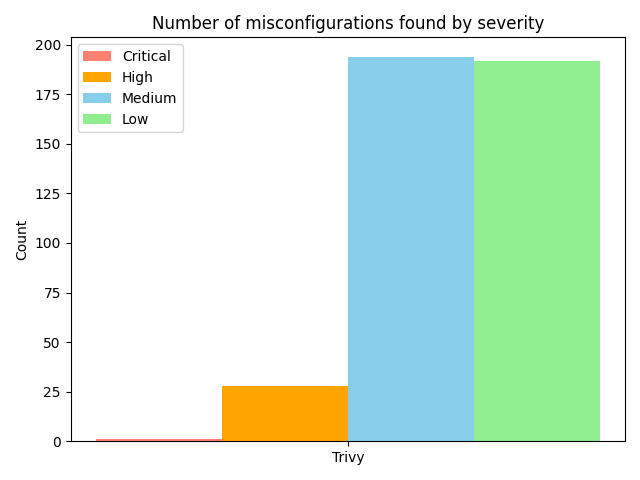
\includegraphics[width=0.5\textwidth]{images/trivy-misconfigurations.png}
        \caption{Trivy's misconfiguration scan performance.}
		\label{img:trivy-misconfigurations}
	\end{center}
\end{figure}

Figure~\ref{fig:success-rates} displays the percentage of successfully passed tests executed by each scanner. On the left side we can see the results with manual checks, the right side shows the results excluding the manual tests. As we can see, most of the automated checks performed by the Kube-bench have failed. This is due to the Kube-bench not separating the results by the target. Even if one of the RBAC configuration files is invalid, the whole test is marked as failed, whereas other scanners distinguish between different targets and provide results for them separately. 

Kubescape has a broader coverage between different domains of misconfigurations than Prowler or Trivy. Therefore, it has a lower success rate as many of those misconfigurations not covered by the other scanners have been detected as failures by Kubescape. Even though we have discovered a few false positives in Trivy results, it has the highest overall success rate. This, however, does not mean that it has missed some important misconfigurations. Looking at the Fig~\ref{img:number-of-checks}, we see that Trivy scan includes a lot of checks that do not fail on the default configuration and distinguishes between all of the target resources. 

\begin{figure}[!h]
        \centering
        \begin{subfigure}{.4\textwidth}
        \centering
        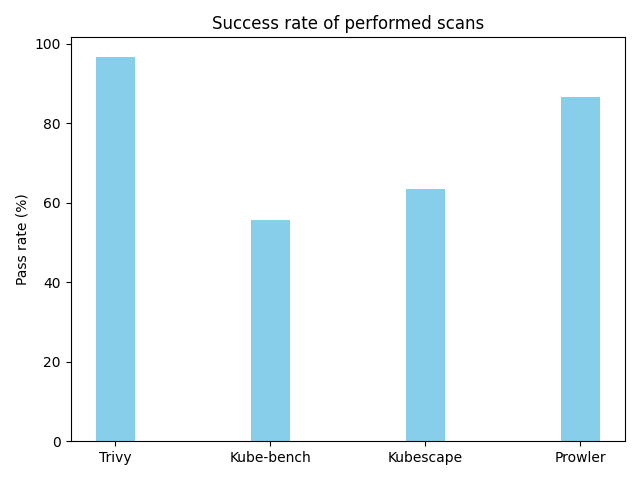
\includegraphics[width=\textwidth]{images/success-rate.png}
        \caption{Success rate of the tests, including those manually performed.}
        \label{img:success-rate-with-manual}
        \end{subfigure}
        \begin{subfigure}{.4\textwidth}
        \centering
        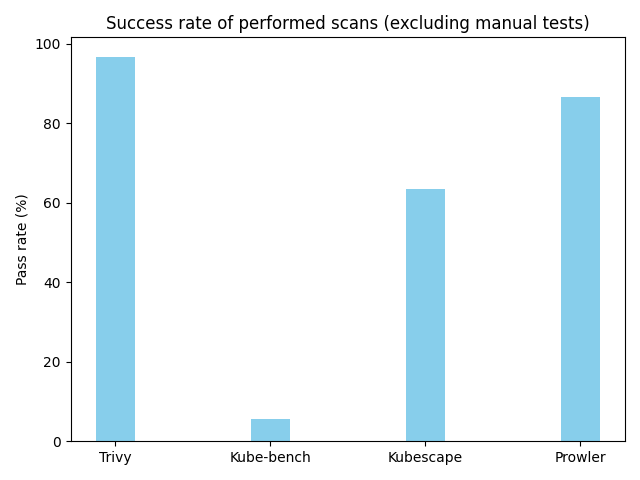
\includegraphics[width=\textwidth]{images/success-rate-no-manual.png}
        \caption{Success rate of the tests, excluding manually performed tests.}
        \label{img:success-rate-no-manual}
        \end{subfigure}
        \caption{Success rate of different scanners, showing the percentage of successfully passed tests.}
        \label{fig:success-rates}
\end{figure}

Trivy's scan did over than 12000 checks on our small demo cluster. Trivy has the most thorough ruleset, which checks for singular misconfigurations. For instance, while most of the scanners check for added pod capabilities in one rule, Trivy includes a separate rule for each added capability.

Trivy and Kubescape show similar results in vulnerability scanning. Kubescape has detected a few additional vulnerbilities that were not detected by Trivy in low severity category. Looking at the Fig~\ref{img:vulnerabilites-by-application-type}, we can see that Trivy performs better in our frontend NodeJS applications, where it has found slightly more vulnerabilities. Nevertheless, Kubescape has been able to detect a few critical vulnerabilities in our backend applications, that were completely missed by the Trivy. Upon further investigation we discover that \textbf{tomcat-embed-core}, \textbf{tomcat-embed-el} and \textbf{tomcat-embed-websocket} packages have 13 critical vulnerabilites and yet none of them were detected by the Trivy. 

\begin{figure}[!hbt]
	\begin{center}
		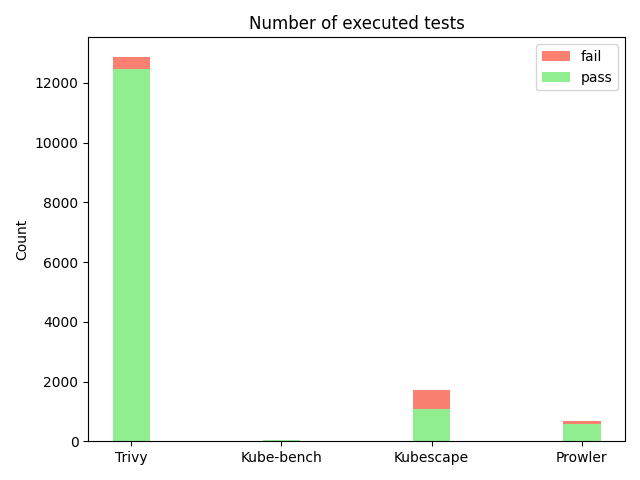
\includegraphics[width=0.5\textwidth]{images/number-of-checks.png}
        \caption{Quantity of executed tests by each scanner.}
		\label{img:number-of-checks}
	\end{center}
\end{figure}

\begin{figure}[!h]
        \centering
        \begin{subfigure}{.4\textwidth}
        \centering
        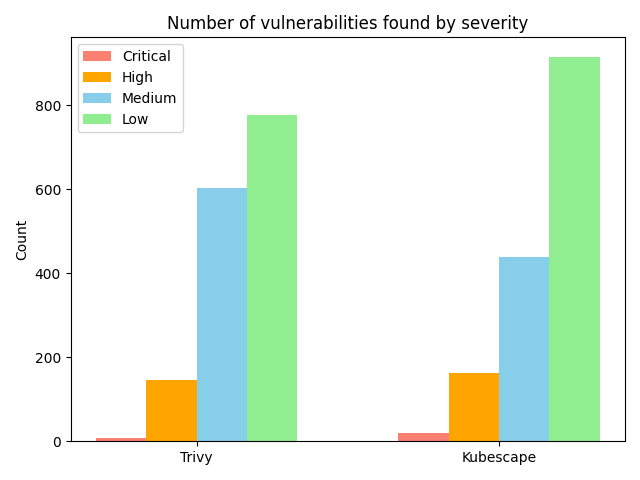
\includegraphics[width=\textwidth]{images/vulnerabilities-by-severity.png}
        \caption{Comparison of vulnerability count by severity.}
        \label{img:vulnerabilites-by-severity}
        \end{subfigure}
        \begin{subfigure}{.4\textwidth}
        \centering
        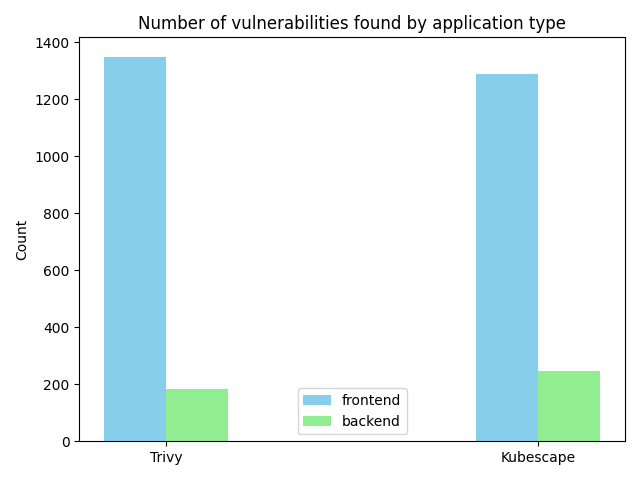
\includegraphics[width=\textwidth]{images/vulnerabilities-by-application-type.png}
        \caption{Comparison of vulnerability count by application type.}
        \label{img:vulnerabilites-by-application-type}
        \end{subfigure}
        \caption{Number of vulnerabilites found in demo applications by Trivy and Kubescape.}
        \label{fig:vulnerability-comparison}
\end{figure}

Based on these results we can conclude that Kubescape would be the best choice for a cloud security engineer. It has a broad feature set, which includes both vulnerability and misconfiguration scanning. It shows the best performance in vulnerability scanning and was able to detect most of our pre-planted misconfigurations. Since it is not extendable, our recommendation would be to use it in conjuction with other security tool that is able to detect missing preemption policy labels. There were no such tool among those selected for the research, unfortunately. None of the tools could detect an exposed secret inside the container when executed in a cluster scan mode, but this threat should be detected on the build step of the CI/CD pipeline or at the image registry level.

The assessment was also carried out on the enterprise-level cluster within one of the IBM projects. Upon agreement with the customer, we can only publish some of the security threats. The cluster has over 125 namespaces with more than 2000 workloads. Trivy was unable to finish neither of the full-cluster scans, it crashed with timeout exception after several hours of execution. When executed against a single namespace, it produced a report after two hours and detected 19 misconfigurations and over 7000 vulnerabilites inside the containers. Most probably, Trivy does a thorough container image scan, which severely affects its performance. Kubescape managed to finish the scan in a few minutes, detecting over 20000 misconfigurations. Prowler has detected about 5000 misconfigurations in that cluster. Among those were added capabilities for logging agents and IBM proxy workloads, network sharing and privileged containers on the master node proxies and CSI volume drivers. The aforementioned threats, though present an actual risk, can be neglected as they are unavoidable for those workloads. They account for about 70\% of those misconfigurations and we would expect them to be ignored when official support for IBM Cloud is added. Among the business workloads there were containers with root privileges and containers with missing security profiles, none other misconfigurations were found there. Kube-bench CIS Benchmark checks have detected 9 failures: \lstinline{cluster-admin} role usage, default service account usage, mounting of service account tokens, create pods access, wildcards in Roles and ClusterRoles, access to the secrets, incorrect permissons on the 3 node configuration files. 

Figure~\ref{fig:ibm-cloud-results} exhibits the results obtained on the IBM Cloud cluster in comparison
with locally produced ones. Even though the number of executed tests is significantly higher in the IBM Cloud cluster, pass rates do not vary significantly between Rancher Desktop and IBM Cloud results. Thus, we can assume, that IBM Cloud cluster instance is predisposed with similar misconfigurations as our local cluster, but on a larger scale.

\begin{figure}[!h]
        \centering
        \begin{subfigure}{.45\textwidth}
        \centering
        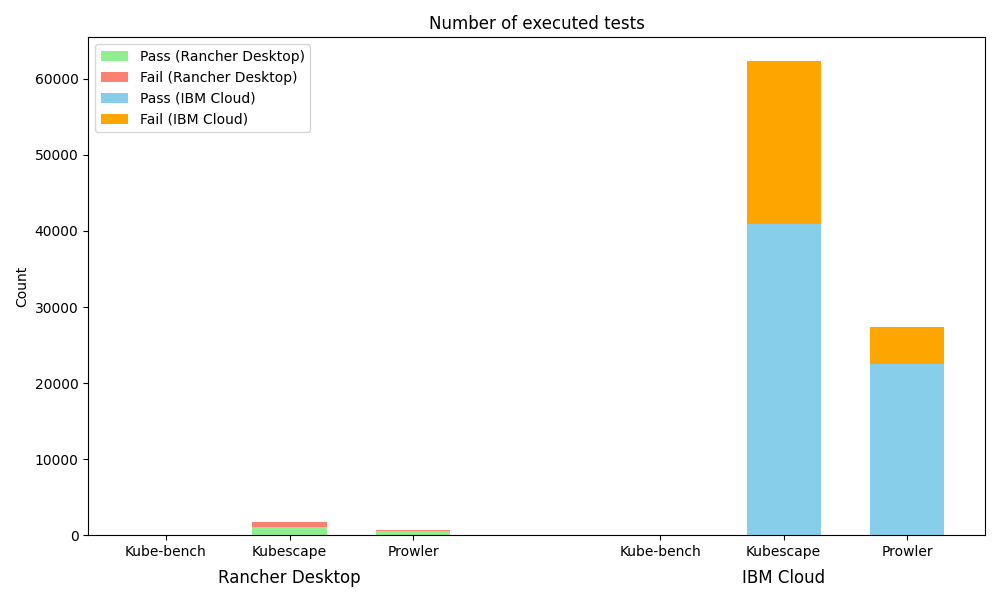
\includegraphics[width=\textwidth]{images/ibm-cloud-count-comparison.png}
        \caption{Comparison by the number of misconfigurations found.}
        \label{img:vulnerabilites-by-severity}
        \end{subfigure}
        \begin{subfigure}{.45\textwidth}
        \centering
        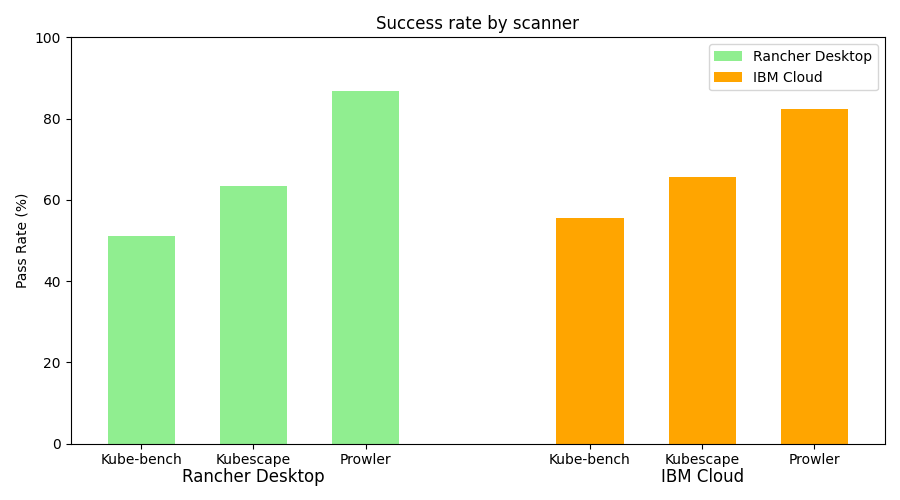
\includegraphics[width=\textwidth]{images/ibm-cloud-success-rate-comparison.png}
        \caption{Comparison of pass rates for the selected scanners.}
        \label{img:vulnerabilites-by-application-type}
        \end{subfigure}
        \caption{IBM Cloud results compared with Rancher Desktop.}
        \label{fig:ibm-cloud-results}
\end{figure}

Finally, as we discovered that Kubescape cannot be extended and there are only two missing checks, we decided to not create a framework of our own, but to create a tool that would aggregate multiple scanners covering the whole range of security domains. A cloud solution for automatic aggregation and parsing of the Kubernetes scanner results has been developed. It is able to parse the reports of multiple scanners and present the results in structured and easily managable format in form of a security dashboard. This dashboard is implemented in a way that would allow further extension with the new scanners. Scan jobs can be directly triggered via the dashboard and the parsing is triggered automatically as the job finishes. Users are able to review misconfigurations and vulnerabilities found by the scanners, search through them, mark failed checks as resolved, remove unwanted items from the results and generate JSON reports. This solution is designed for a DevSecOps specialist and significantly improves his work efficiency by automating multiple processes.

In the future it would be necessary to integrate Kubescape Operator into the dashboard deployment, so that full potential of Kubescape can be achieved. Without the Operator Kubescape can only perform a handful of controls. Integrating AI into the dashboard would bring a lot of benefits: we could filter out duplicates produced by different scanners and generate summaries with the most critical findings. At this moment, duplicates are hard to recognize as different scanners use different internal ids for misconfigurations and classify them differently. But AI could, perhaps, detect duplciates based on the combination of properties. Automatic failure mitigation is a controversal subject. Usually, automatic configuration changes are not desired, but with proper caution and verification this could be accepted. Therefore, this could be a potential extension of the dashboard. Less far-fetched feature is the generation of PDF or CSV reports. This can be implemented in such a way that user can choose in which format to download the report. Lastly, ``Statistics'' tab can be reworked into a separate page and additional charts could be added there. The most interesting of them would be the chart that showcases the trent in misconfiguration or vulnerability count over the time based on the generated reports.